\documentclass[12pt, a4paper]{article}
\usepackage[utf8]{inputenc}
\usepackage{fontenc}
\usepackage[dvipsnames]{xcolor}
\usepackage{hyperref}
\usepackage[english]{babel}
\usepackage[inline]{enumitem}
\usepackage{graphicx}
\usepackage{cleveref}
\usepackage{listings}

\definecolor{codegreen}{rgb}{0,0.6,0}
\definecolor{codegray}{rgb}{0.5,0.5,0.5}
\definecolor{codepurple}{rgb}{0.58,0,0.82}
\definecolor{backcolour}{rgb}{0.95,0.95,0.92}

\lstdefinestyle{mystyle}{
    backgroundcolor=\color{backcolour},   
    commentstyle=\color{codegreen},
    keywordstyle=\color{magenta},
    numberstyle=\tiny\color{codegray},
    stringstyle=\color{codepurple},
    basicstyle=\ttfamily\footnotesize,
    breakatwhitespace=false,         
    breaklines=true,                 
    captionpos=b,                    
    keepspaces=true,                 
    numbers=left,                    
    numbersep=5pt,                  
    showspaces=false,                
    showstringspaces=false,
    showtabs=false,                  
    tabsize=2
}

\lstset{style=mystyle}

\lstdefinelanguage{Kotlin}{
  comment=[l]{//},
  commentstyle={\color{gray}\ttfamily},
  emph={filter, first, firstOrNull, forEach, lazy, map, mapNotNull, println},
  emphstyle={\color{OrangeRed}},
  identifierstyle=\color{black},
  keywords={!in, !is, abstract, actual, annotation, as, as?, break, by, catch, class, companion, const, constructor, continue, crossinline, data, delegate, do, dynamic, else, enum, expect, external, false, field, file, final, finally, for, fun, get, if, import, in, infix, init, inline, inner, interface, internal, is, lateinit, noinline, null, object, open, operator, out, override, package, param, private, property, protected, public, receiveris, reified, return, return@, sealed, set, setparam, super, suspend, tailrec, this, throw, true, try, typealias, typeof, val, var, vararg, when, where, while},
  keywordstyle={\color{NavyBlue}\bfseries},
  morecomment=[s]{/*}{*/},
  morestring=[b]",
  morestring=[s]{"""*}{*"""},
  ndkeywords={@Deprecated, @JvmField, @JvmName, @JvmOverloads, @JvmStatic, @JvmSynthetic, Array, Byte, Double, Float, Int, Integer, Iterable, Long, Runnable, Short, String, Any, Unit, Nothing},
  ndkeywordstyle={\color{BurntOrange}\bfseries},
  sensitive=true,
  stringstyle={\color{ForestGreen}\ttfamily},
}

\setlist[enumerate,1]{label=\arabic*}
\setlist[enumerate,2]{label=\theenumi.\arabic*}
\setlist[enumerate,3]{label=\theenumii.\arabic*}
\setlist[enumerate,4]{label=\theenumiii.\arabic*}

\graphicspath{ {res/} }
% version
\newcommand{\versionmajor}{0}
\newcommand{\versionminor}{1}
\newcommand{\versionpatch}{2}
\newcommand{\version}{\versionmajor.\versionminor.\versionpatch}
\typeout{Document version: \version}

\title{\LARGE
    Middleware for the communication between Distributed Agents in JaKtA \\ \small Project for the course \textit{Intelligent Systems Engineering}
}

\author{
   Angela Cortecchia \\ \small angela.cortecchia@studio.unibo.it
    \and
    Leonardo Micelli \\ \small leonardo.micelli@studio.unibo.it
    \and
    Filippo Vissani \\ \small filippo.vissani@studio.unibo.it
}

\date{\small Anno accademico 2022/2023}
\makeindex

\begin{document}
\maketitle

\clearpage
\tableofcontents
\clearpage
\section{Introduction}

\subsection{Agents}

\subsubsection{Definition}
An agent is an autonomous computational entity endowed with decision-making and independent execution capabilities. Agents are designed to operate in a specific environment, assuming defined responsibilities and tasks. The key characteristic of an agent is its autonomy, which means it can make decisions independently, without requiring external intervention for every action undertaken. This computational autonomy implies intrinsic proactivity, wherein agents don't passively await events but actively act to change the state of the Multi-Agent System (MAS).

A MAS, or Multi-Agent System, is a computational system composed of multiple autonomous agents that interact with each other to achieve common or individual goals. In a MAS, each agent is an autonomous entity with perception, reasoning, decision-making, and action capabilities. Agents in a MAS can operate independently and, simultaneously, collaborate to address complex problems or achieve goals that may be difficult or impossible for a single agent to accomplish.

A crucial aspect is the situational nature of agents, meaning their actions depend on the context in which they find themselves. Agents, by interacting with each other and the surrounding environment, become inherently social entities. This sociality emerges because autonomy makes sense only when an agent is immersed in a society of agents, highlighting the absence of truly autonomous agents in isolation. Interaction occurs through the exchange of knowledge and information, while the proactivity of agents drives them to change the state of the MAS, influencing other agents or the environment. In this context, agents become autonomous, interactive, and social components that, through their self-regulation capabilities, are essential for managing complex systems.

\subsubsection{The Framework Belief-Desire-Intention}
The Belief-Desire-Intention (BDI) framework is widely accepted as one of the most popular and successful frameworks in the field of agent technology. Defined by Rao and Georgeff, the framework is based on three key concepts: belief, desire, and intention. Agents that adhere to this framework are commonly referred to as BDI agents.
The following are the characteristics of the framework:
\begin{itemize}
    \item \textbf{Belief}: To make decisions, agents must have a representation of the world in which they exist. Beliefs are the knowledge about the environment that agents gather and can store as part of their belief base.
    \item \textbf{Desire}: Desires represent the main goals of the system. Agents have a set of plans at their disposal that they can use to achieve their goals, and the choice of the most suitable plan depends on the current situation of the agent and the environment.
    \item \textbf{Intention}: Intentions capture the deliberative component of the system. They represent the actions to which the agent has committed to executing to achieve its goals. Intentions keep track of the progress of actions and changes in the environment during execution.
\end{itemize}

\subsection{JaKtA}
JaKtA\cite{10.1007/978-3-031-43264-4_4} is a library that provides the capability to develop agents that perceive and act within a shared environment and communicate with each other through a message-based communication system.

The library offers a framework for building multi-agent systems (MAS) composed of agents conforming to the Belief-Desire-Intention (BDI) model and inspired by the implementation of Jason\cite{Bordini2005}. A Multi-Agent System consists of two fundamental entities:

\begin{itemize}
    \item \textbf{Agents}: Agents are the main entities of the library.
    \item \textbf{Environment}: The environment in which agents live.
\end{itemize}

During their execution, agents in a MAS autonomously observe the environment's state and choose to act based on perceived information. Their actions can influence the state of the environment, and this change will be perceived by all other agents operating on it. Agents are equipped with goals that they are committed to achieving, contributing to the overall goal of the Multi-Agent System. As for the environment, a user can:

\begin{itemize}
    \item Create an environment.
    \item Add functionalities to the environment, such as:
    \begin{itemize}
        \item Define the actions that agents within the environment can use.
        \item Define the state of the environment, including the set of information that agents can perceive and potentially modify.
    \end{itemize}
    \item Add and remove agents from the environment.
\end{itemize}

Moreover, agents located in the same environment can communicate with each other through messages. Messages allow agents to share information about their state or share the completion of a goal, making the Multi-Agent System a true society of agents. Regarding agents, a user can:

\begin{itemize}
    \item Create and customize agents' behavior, following the BDI model.
    \item Add actions related to an agent.
    \item Customize the behavior of agents during their execution.
\end{itemize}

The library enables users to define how their BDI agents will be executed. This means that the same agents can be executed either in a single thread or among multiple threads, in a nearly transparent manner. To enable the MAS to do this, users must define its execution model, i.e., how its agents are executed.

\subsection{Middleware for Communication among Distributed Agents}

The current implementation of JaKtA focuses on managing multi-agent systems locally, limiting consideration to agents distributed over a network. To address this limitation and enable effective communication among distributed agents, the introduction of a dedicated middleware is proposed.
A middleware for communication among distributed agents would act as an intermediate layer between the agents themselves and the network, providing an abstraction that makes the complexities of distributed communication transparent to the programmer. The middleware aims to handle the sending and receiving of messages between agents located on different machines, ensuring information consistency.
The middleware would be responsible for establishing and maintaining connections between distributed agents. This includes managing communication protocols, handling lost connections, and addressing any delays or transmission errors.
Implementing middleware for communication among distributed agents would enhance JaKtA's ability to support scenarios where agents operate on heterogeneous or geographically distant networks. This would allow the creation of multi-agent systems that can collaborate and coordinate their actions on a larger scale, opening up new application possibilities for the JaKtA library.

\clearpage
\section{Analisi dei Requisiti}

% Is there any implicit requirement hidden within this project's requirements?
%
% Is there any implicit hypothesis hidden within this project's requirements?
%
% Are there any non-functional requirements implied by this project's requirements?

% What model / paradigm / technology is the best suited to face this project's requirements?
%
% What's the abstraction gap among the available models / paradigms / technologies and the problem to be solved?

\subsection{Goal}

Il goal principale del progetto è quello di estendere la libreria JaKtA e il relativo framework per la costruzione di Sistemi Multi-Agenti,
con la creazione di un middleware per l'interazione tra sistemi multi-agente distribuiti.

\subsection{Requisiti}
A partire dal goal principale del progetto, sono stati individuati diversi requisiti funzionali:

\begin{enumerate}
      \item Gestione della distribuzione degli agenti:
            \begin{enumerate}
                  \item  Il middleware deve supportare la distribuzione degli agenti su macchine eterogenee,
                        consentendo la loro esecuzione coordinata su diverse posizioni geografiche.
            \end{enumerate}

      \item Implementazione di un meccanismo di dispatch dei messaggi tra i vari agenti:
            \begin{enumerate}
                  \item Il middleware deve essere composto da un broker:
                        \begin{enumerate}
                              \item Il broker deve consentire l'aggiunta di publisher associati a un determinato topic.
                              \item Il broker deve permettere la rimozione di publisher associati a un topic specifico.
                              \item Il broker deve supportare l'aggiunta di subscriber associati a un determinato topic.
                              \item Il broker deve permettere la rimozione di subscriber associati a un topic specifico.
                              \item Il broker deve fornire l'elenco di tutti i topic disponibili.
                              \item Il sistema deve utilizzare strutture dati sincronizzate per gestire in modo sicuro e concorrente l'associazione di publishers e subscribers ai topic.
                        \end{enumerate}
                  \item Il middleware deve essere composto da un client:
                        \begin{enumerate}
                              \item Il client deve fornire la funzionalità di pubblicare un messaggio su un determinato topic.
                              \item Il client deve offrire la possibilità di sottoscriversi a un topic specifico.
                              \item Il sistema deve consentire al client di effettuare una trasmissione broadcast, inviando un messaggio a tutti i client connessi.
                              \item  Il client deve essere in grado di stabilire e gestire connessioni WebSocket verso un server specificato tramite host e porta.
                        \end{enumerate}
            \end{enumerate}

      \item  Comunicazione Distribuita e Coordinazione
            \begin{enumerate}
                  \item  Il middleware deve gestire la comunicazione distribuita tra agenti, facilitando
                        lo scambio di messaggi e la coordinazione delle attività.
                  \item Deve supportare la sincronizzazione degli agenti distribuiti per garantire
                        un'interazione coesa e coordinata.
            \end{enumerate}
\end{enumerate}

% \subsubsection{Requisiti non funzionali}

% \begin{enumerate}
%     \item  Il sistema deve essere scalabile, consentendo l'aggiunta di nuovi client e broker senza compromettere le prestazioni generali del sistema.
%     \item
%     \item
% \end{enumerate}
\clearpage
\section{Design}
In questa sezione esporremo il design del progetto, partendo dalle decisioni prese in ambito architetturale e proseguendo
col design di dettaglio.

\subsection{Design Architetturale}
Come precedentemente illustrato nei capitoli precedenti, il progetto si propone di sviluppare un meccanismo per la creazione di sistemi multi-agente distribuiti utilizzando \textit{JaKTa}.
Il gruppo ha deciso di raggiungere questo obiettivo fornendo un'estensione del framework e del suo Domain Specific Language il più minimale possibile.
Dal punto di vista architetturale, il progetto si colloca come modulo a sé stante, come mostrato nella figura \ref{fig:architecture}:

\begin{figure}[ht!]
    \centering
    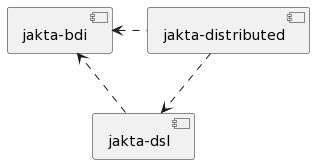
\includegraphics[width=0.8\textwidth]{figures/general-architecture.png}
    \caption{Architettura del progetto}
    \label{fig:architecture}
\end{figure}

In particolare, il modulo sviluppato è formato da tre componenti principali, come mostrato nella figura \ref{fig:detailed-architecture}:

\begin{figure}[ht!]
    \centering
    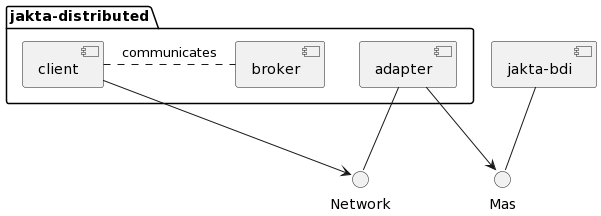
\includegraphics[width=0.8\textwidth]{figures/detailed-architecture.png}
    \caption{Architettura del modulo sviluppato}
    \label{fig:detailed-architecture}
\end{figure}

Dei moduli rappresentati in figura \ref{fig:detailed-architecture}, il modulo \textit{Adapter} è quello che definisce e contiene tutti i concetti da implementare per realizzare l'obiettivo di progetto,
mentre i moduli \textit{Client} e \textit{Broker} forniscono una prima implementazione della logica di comunicazione tra i sistemi multi-agente distribuiti.\\

Come anticipato in precedenza, il progetto presenta anche un'estensione del Domain Specific Language di JaKTa, la cui struttura è rappresentata nella figura \ref{fig:dsl-architecture}.

\begin{figure}[ht!]
    \centering
    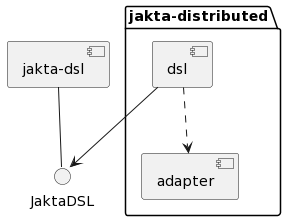
\includegraphics[width=0.8\textwidth]{figures/dsl-architecture.png}
    \caption{Architettura del Domain Specific Language}
    \label{fig:dsl-architecture}
\end{figure}

\subsubsection{Architettura di Rete}

Il diagramma dei componenti presentato in Figura \ref{fig:network-architecture} offre una panoramica dell'architettura di rete.
Il \textit{Broker} espone quattro interfacce: le interfacce \texttt{/subscribe/{topic}} e \texttt{/publish/{topic}} consentono rispettivamente la sottoscrizione e la pubblicazione su \textit{topic} specifici, mentre l'interfaccia \texttt{/topics} fornisce un mezzo per recuperare l'elenco dei \textit{topic} disponibili. Inoltre, l'interfaccia \texttt{/subscribe-all/\{except...\}} offre la possibilità di sottoscrivere tutti i \textit{topic} tranne quelli specificati. Il \textit{Dmas}, d'altra parte, si connette al \textit{Broker} attraverso queste interfacce, sfruttandole per sottoscrivere, pubblicare e ottenere informazioni dagli altri \textit{Dmas}. Questo setup permette la gestione delle comunicazioni distribuite, con il \textit{Broker} che funge da fulcro centrale per agevolare la sottoscrizione, la pubblicazione e la gestione dei \textit{topic} all'interno del sistema.

\begin{figure}[ht!]
    \centering
    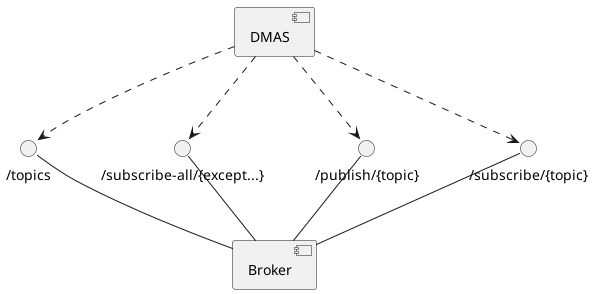
\includegraphics[width=0.8\textwidth]{figures/network-architecture.png}
    \caption{Architettura di rete}
    \label{fig:network-architecture}
\end{figure}

\subsection{Design di Dettaglio}
La soluzione proposta consiste nell'implementazione di una versione alternativa dell'interfaccia \textit{Mas}, chiamata \textit{Dmas}, da utilizzare in contesti distribuiti.
Questa estensione dovrà comportarsi come un Mas, ma in aggiunta dovrà essere in grado di comunicare con altri Dmas attraverso la rete.

\subsubsection{Adapter}
Questo modulo si occupa di definire i concetti di:
\begin{itemize}
    \item \textbf{Dmas}: rappresenta un sistema multi-agente distribuito, cioè che può comunicare con altri sistemi Dmas attraverso la rete.
    \item \textbf{Network}: incapsula la logica di comunicazione tra Dmas attraverso la rete.
    \item \textbf{RemoteService}: rappresenta un agente remoto, cioè un agente che appartiene ad un Dmas diverso da quello corrente, ma contattabile attraverso la rete.
\end{itemize}

Le relazioni tra questi concetti sono esemplificate dal diagramma delle classi in figura \ref{fig:class-dmas}.

\begin{figure}[ht!]
    \centering
    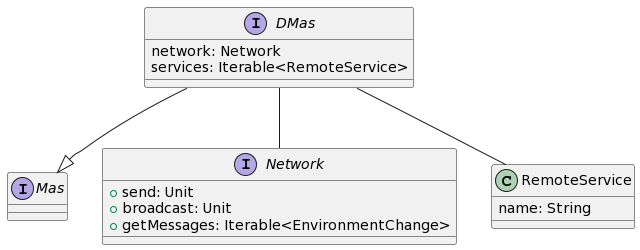
\includegraphics[width=0.8\textwidth]{figures/class-dmas.png}
    \caption{Diagramma delle classi del modulo Adapter}
    \label{fig:class-dmas}
\end{figure}

\subsubsection{Broker}

Il diagramma delle classi del broker (Figura \ref{fig:broker-class-diagram}) presenta una struttura organizzata e modulare. Nel package \texttt{model}, sono definite due interfacce chiave: \texttt{Cache<T>} per la registrazione, la liberazione e la lettura di dati associati a un \textit{topic}, e \texttt{SubscriptionManager<T>} per gestire la sottoscrizione, l'aggiunta e la rimozione di \textit{publisher} e \textit{subscriber}, nonché l'ottenimento dei \textit{topic} disponibili e dei \textit{subscriber} associati a un \textit{topic}. Il package \texttt{plugins} include le classi \texttt{Routing} e \texttt{Websockets}, che vengono utilizzate per la definizione delle \textit{API Web}

\begin{figure}[ht!]
    \centering
    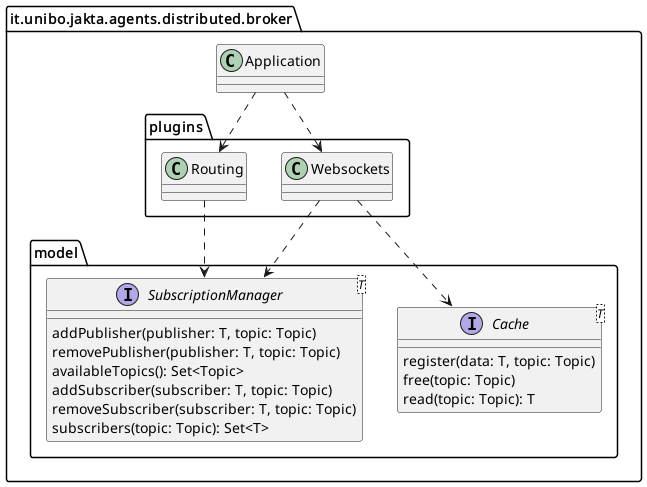
\includegraphics[width=0.8\textwidth]{figures/broker-class-diagram.png}
    \caption{Diagramma delle classi del \textit{Broker}}
    \label{fig:broker-class-diagram}
\end{figure}

\subsection{Comportamento}
Il comportamento delle varie componenti del sistema può essere descritto attraverso i seguenti passaggi:

\subsubsection{Inizializzazione del Sistema}

\begin{enumerate}
    \item istanziazione di una Network;
    \item connessione da parte della Network al broker;
    \item definizione dei RemoteService di interesse;
    \item istanziazione di un Dmas;
    \item per ogni RemoteService, il Dmas si sottoscrive ai topic di interesse;
    \item esecuzione del dispatch della ExecutionStrategy scelta per il Dmas;
\end{enumerate}

Queste attività sono illustrate in figura \ref{fig:initialization}.

\begin{figure}
    \centering
    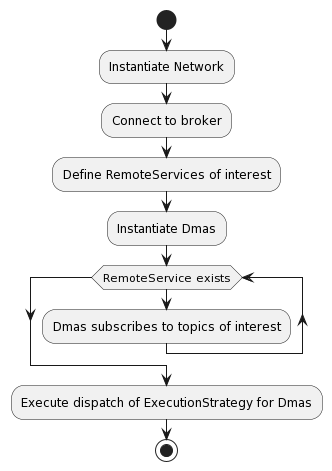
\includegraphics[width=0.8\textwidth]{figures/activity-dmas.png}
    \caption{Inizializzazione del sistema}
    \label{fig:initialization}
\end{figure}

\subsubsection{Ciclo di Esecuzione del Dmas}

\begin{enumerate}
    \item il Dmas raccoglie tutti gli eventi esterni ricevuti dalla Network, ossia i messaggi pubblicati dai RemoteService a cui si è sottoscritto e le eventuali notifiche di disconnessione di un RemoteService, sotto forma di EnvironmentChange;
    \item gli eventi esterni vengono concatenati alla coda degli EncironmentChange interni del Dmas;
    \item ad uno ad uno, gli EnvironmentChange vengono processati dal Dmas. Nel caso in cui l'evento consista nell'inviare un messaggio ad un RemoteService o un broadcast, il messaggio viene inviato alla Network, che si occuperà di inoltrarlo al broker;
\end{enumerate}

Queste attività sono illustrate in figura \ref{fig:execution}.

\begin{figure}
    \centering
    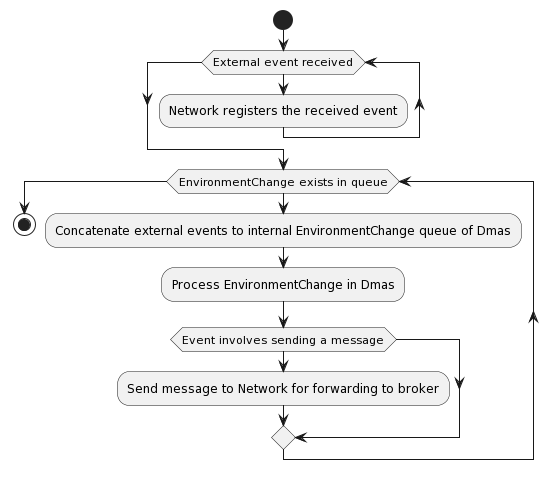
\includegraphics[width=0.8\textwidth]{figures/activity-applychanges.png}
    \caption{Ciclo di esecuzione del Dmas}
    \label{fig:execution}
\end{figure}

\subsection{Interazioni}
Il modello di interazione tra i vari Dmas collegati alla rete è di tipo publish-subscribe: ogni Dmas, che assume il ruolo di client, può sottoscrivere ad uno o più topic, e può pubblicare messaggi su uno o più topic.
I messaggi pubblicati su un topic vengono ricevuti da tutti i client che si sono sottoscritti a quel topic.
Il broker, che assume il ruolo di server, si occupa di gestire la comunicazione tra i client, in particolare si occupa di:
\begin{itemize}
    \item ricevere i messaggi pubblicati dai client;
    \item inviare i messaggi ai client sottoscritti ai topic corrispondenti;
    \item gestire le connessioni e le disconnessioni dei client.
    \item gestire la sottoscrizione dei client ai vari topic.
\end{itemize}

Il comportamento di clients e broker in situazioni di broadcast e invio di messaggi con singolo destinatario è illustrato nelle figure \ref{fig:interaction-broadcast} e \ref{fig:interaction-sendmessage}.

\begin{figure}[ht!]
    \centering
    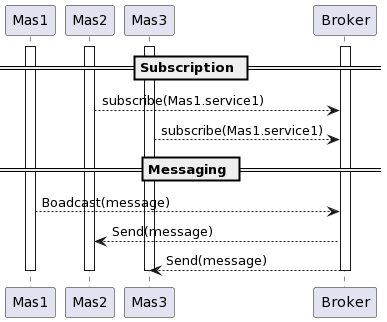
\includegraphics[width=0.8\textwidth]{figures/interaction-broadcast.png}
    \caption{Interazione tra DMas, client e broker in caso di broadcast}
    \label{fig:interaction-broadcast}
\end{figure}

\begin{figure}[ht!]
    \centering
    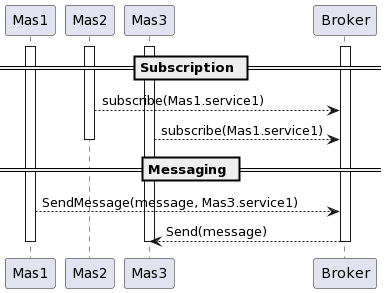
\includegraphics[width=0.8\textwidth]{figures/interaction-sendmessage.png}
    \caption{Interazione tra DMas, client e broker in caso di invio di messaggio con singolo destinatario}
    \label{fig:interaction-sendmessage}
\end{figure}

\clearpage
\section{Implementation Details}

Just report interesting / non-trivial / non-obvious implementation details.

This section is expected to be short in case some documentation (e.g. Javadoc or Swagger Spec) has been produced for the software artefacts.
%
This this case, the produced documentation should be referenced here.

\clearpage
\section{Self-assessment / Validation}

Choose a criterion for the evaluation of the produced software and \textbf{its compliance to the requirements above}.

Pseudo-formal or formal criteria are preferred.

In case of a test-driven development, describe tests here and possibly report the amount of passing tests, the total amount of tests and, possibly, the test coverage.
\clearpage
\section{Usage Examples}

Show how to use the produced software artefacts.

Ideally, there should be at least one example for each scenario proposed above.
\clearpage
\section{Conclusioni}
L'obiettivo di questo progetto era dare la possibilità agli utenti del \textit{framework} JaKtA la possibilità di creare sistemi multi-agente distribuiti in modo semplice e veloce, con il minore \textit{overhead} possibile.

È stata quindi sviluppata un'estensione del \textit{framework} che fornisce una nuova implementazione del concetto di sistema multi-agente, in grado di comunicare con gli altri sistemi con modello di comunicazione asincrono \textit{publish-subscribe}.

Questo modello di comunicazione è stato implementato attraverso il \textit{framework} Ktor ed il protocollo \textit{WebSocket}.

Il team ritiene che l'obiettivo sia stato raggiunto, tuttavia è conscio di alcuni possibili miglioramenti alla soluzione proposta, che verranno discussi nella sezione successiva.

In conclusione, il progetto ha costituito una buona occasione per approfondire le conoscenze acquisite nell'ambito dei sistemi multi-agente, della programmazione \textit{agent-oriented} e dei sistemi distribuiti.


\subsection{Sviluppi Futuri}
Il team ritiene che il progetto abbia raggiunto gli obiettivi prefissati, tuttavia è consapevole che la soluzione proposta possa essere migliorata in diversi aspetti, alcuni dei quali vengono elencati di seguito:

\begin{itemize}
    \item \textbf{Supporto a più protocolli di comunicazione}: attualmente il \textit{framework} supporta un solo protocollo di comunicazione, ovvero \textit{WebSocket}. Tuttavia sarebbe interessante
    fornire agli utenti la possibilità di scegliere tra diversi protocolli, come ad esempio \textit{MQTT}. L'architettura del progetto permetterebbe agevolmente l'aggiunta del supporto ad \textit{MQTT}
    tramite l'implementazione di una nuova \texttt{Network} ed eventualmente un nuovo \textit{broker}.
    \item \textbf{Gestione dell'univocità dei nomi dei servizi remoti}: come già accennato nella sezione "Dettagli Implementativi", il \textit{framework} non fornisce alcun meccanismo per garantire
    l'univocità dei nomi dei servizi remoti. Una possibile soluzione può essere quella di aggiungere uno step di coordinazione al momento della connessione al \textit{broker}, in modo da dare la possibilità ai
    \textit{Dmas} di registrare i propri servizi e verificare che il nome scelto non sia già stato utilizzato.
\end{itemize}



\bibliographystyle{plain}
\bibliography{bibliography}

\end{document}
